\documentclass{article}
\usepackage{amsmath}
\usepackage{amssymb}
\usepackage{graphicx}
\usepackage{hyperref}
\usepackage[version=4]{mhchem}


\begin{document}
\(A B\) is the diameter of circle \(O . C\) is a point on the circumference of circle \(O . A D\) is perpendicular to the tangent line drawn through \(C\). Show that \(A C\) is the angle bisector of \(\angle D A B\).

Solution:
Connect \(C O\). Since \(O A=O C, \angle O A C=\angle O C A=\alpha\).\\
\centering
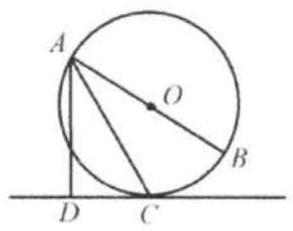
\includegraphics[width=\textwidth]{images/148(4).jpg}

Since \(A D \perp C D\) and \(O C \perp C D, A D / / O C\) and \(\angle D A C=\) \(\angle O C A=\alpha\) (alternate interior angles).\\
So \(A C\) is the angle bisector of \(\angle D A B\).\\
\centering
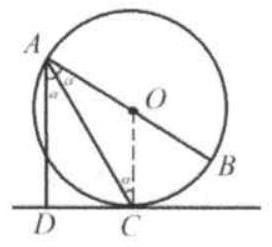
\includegraphics[width=\textwidth]{images/148(1).jpg}


\end{document}
